\documentclass{ProcISPRAS}

% Page geometry. Nearly A5, but not exactly
\usepackage[papersize={14.86cm,21cm},
            left=1.5cm, % 1.4cm
            right=1cm, % 1.5cm
            top=0.8cm, % 0.5cm
            bottom=1cm, % 1.5cm
            includehead,
            headheight=8pt,
            heightrounded,
            headsep=6pt, % 0.4cm
            includefoot,
            footskip=16pt, % I was told that this value should be 9pt. In printed copies of proceedings it is approximately 16pt. Change on your own risk.
]{geometry}

\addbibresource{bibliography.bib}

\usepackage{url}
\usepackage{tikz}
\usepackage{booktabs}
\usepackage{listings}
\usetikzlibrary{positioning}
\usepackage{algorithmicx}
\usepackage{algpseudocode}

\makeatletter
\newenvironment{restoretext}%
    {\@parboxrestore%
     \begin{adjustwidth}{}{\leftmargin}%
    }{\end{adjustwidth}}
\makeatother

\volhead{1}
\issuehead{2}
\pageshead{3--4}
\yearhead{2000}

\setcounter{page}{1} % Set first page number

\date{July 2000}

\newauthor
\inst{1, 2}
\authorname{Bogatenkova A.\,O.}{Богатенкова~А.\,О.}
\email{nastyboget@ispras.ru}

\newauthor
\inst{1}
\authorname{Kozlov I.\,S.}{Козлов~И.\,С.}
\email{kozlov-ilya@ispras.ru}

\newauthor
\inst{1}
\authorname{Belyaeva O.\,V.}{Беляева~О.\,В.}
\email{belyaeva@ispras.ru}

\newauthor
\inst{1, 2}
\authorname{Perminov A.\,I.}{Перминов~А.\,И.}
\email{perminov@ispras.ru}


\affil[1]{Ivannikov Institute for System Programming of the RAS,\\25, Alexander Solzhenitsyn Str., Moscow, 109004, Russia}{Институт системного программирования им. В.П. Иванникова РАН,\\109004, Россия, г. Москва, ул. А. Солженицына, д. 25}

\affil[2]{Lomonosov Moscow State University,\\GSP-1, Leninskie Gory, Moscow, 119991, Russian Federation}{Московский государственный университет имени М.В. Ломоносова,\\119991, Россия, Москва, Ленинские горы, д. 1.}

\title{Logical structure extraction from scanned documents}{Извлечение логической структуры из сканированных документов}

\doi{10.15514/ISPRAS-2000-1(2)-33}
\keywords{machine learning; document structure; natural language processing; OCR.}{машинное обучение; структура документа; обработка естественного языка; OCR.}

\abstract{
There are many scanned documents without a text layer. Understanding the information in such documents may be useful for their analysis, e. g. for the effective search within documents. 
The paper describes pipeline for scanned documents processing. The method based on multiclass classification including headers and lists classes.
Text and bounding boxes for lines were extracted using OCR methods, different features were generated for each line, which were the input of the classifier.
We also made available dataset \cite{data} of documents, which includes bounding boxes and labels for each document line; evaluated the effectiveness of our approach using this dataset and described the possible future work in the field of document processing. }{Большое количество информации представлено в виде сканированных документов без текстового слоя. Зачастую требуется осуществлять быстрый поиск по их содержимому. Знание структуры документов может способствовать более эффективному их анализу.
% OX: Здесь сначала говорится что описан процесс пайплайн, а потом идет "данный метод основан". Нужно определиться что мы сделали пайплайн или метод или и то и то другое. Лучше в статье описан пайплайн обработки сканированных документов, а также разработан метод извлечения структуры сканированных документов с высокой глубиной вложенности.
В статье описан процесс построения пайплайна обработки сканированных документов, а также разработан метод извлечения структуры из них. Данный метод основан на многоклассовой классификации строк документа, в том числе классификации на заголовки и списки.
Пайплайн состоит из извлечения текста и рамок строк документов с помощью методов OCR, формирования признаков и обучения классификатора на данных признаках. Кроме того, размечен и доступен для изучения \cite{data} корпус документов, проведена экспериментальная проверка реализованного метода на данном корпусе и описаны возможности для дальнейшей работы и исследований.}

\begin{document}

\makedoi

\maketitleen

\newpage

\maketitleru

\section{Введение}

Документы имеют опредёленную логическую структуру. Например, законы делятся на главы, статьи, разделы. Научные статьи состоят из аннотации, введения, обзора существующих работ и других секций.  
Информация о логической структуре полезна для автоматического анализа документа. 

Задача автоматического извлечения логической структуры из документов осложняется следующими факторами:

Во-первых, большое количество документов представляет из себя сканированные изображения с бумажных носителей. Такие изображения не содержат текстовый слой, для его извлечения необходимо использовать 
методы обработки изображений. % использовать методы обработки изображений

Во-вторых, зачастую логические части документа выделяются с помощью форматирования: увеличенного размера шрифта, жирности, отступов. Такая информация помогает читателю лучше понимать структуру документа, автоматическая система также должна учитывать эти признаки. 

%В-третьих, разные типы документов организованым отличным образом. Например, 
В-третьих, разные типы документов организованым отличным образом. Например, научные статьи, финансовые отчёты, законы могут состоять из разных структурных элементов (законы имеют главы, статьи, пункты, подпункты; научные статьи состоят из введения, аннотации, списка литературы). Форматирование и язык документов также могут быть различны (законы, как правило, пишут в 1 колонку, научные статьи -- в 1-2 колонки). Задача создать систему, способную обработать любой тип документа может оказаться слишком сложной, задача построения своей системы для каждого типа документов "с нуля" может оказаться слишком трудоёмкой. Таким образом, наша система должна позволять добавлять поддержку новых типов документов, причём такое добавление не должно быть слишком трудоёмким. 

Многие типы документов имеют требования по оформлению, однако эти требования не являются полностью формализоваными, кроме того составители документов могут от них отклоняться. Поэтому для выделения логической структуры лучше подходят методы машинного обучения.

В данной статье описан метод извлечения структуры документа в виде заголовков, элементов списков и текстовых строк. Каждая строка документа относится к одному из этих трех типов на основе определённых признаков. Для выделения признаков может быть необходима метаинформация, такая как размер и тип шрифта, отступы, междустрочные интервалы и т. д. Поэтому извлечение логической структуры целесообразно делать на этапе анализа изображений.

Данный анализ предполагает следующее: с помощью методов OCR из изображений извлекаются строки документа с текстом и координатами их рамок на изображении. Следующим шагом пайплайна является выделение признаков на основе извлечённых данных. Далее выбранным алгоритмом машинного обучения проводится многоклассовая классификация строк.

Статья организована следующим образом:
глава 2 содержит обзор различных подходов, с помощью которых решается задача выделения структуры документа; в главе 3 раскрывается процесс составления обучающего набора данных, в частности описывается набор документов, используемый при реализации и проверке метода и манифест для разметки данных; в главе 4 рассматривается реализованный метод; в главе 5 показаны результаты экспериментальной проверки метода, сравнение различных методов машинного обучения, анализ ошибок и анализ важности признаков, а в главе 6 представлены краткие выводы и предлагаются возможности для дальнейшей работы и исследований.

\section{Обзор аналогичных работ}

Применяется множество разнообразных подходов \cite{fintoc19daniel, fintoc19tian, deep}, которые позволяют выделять в тексте заголовки и распознавать логическую структуру документов.
Среди подходов можно выделить следующие:
\begin{itemize}
\item на основе оглавления;
\item на основе правил;
\item на основе машинного обучения.
\end{itemize}

\subsection{Извлечение структуры из документов на основе оглавления и правил}

По анализу содержимого и структуре изображений документов проводятся соревнования ICDAR \cite{icdar13, icdar17comp, icdar17}. В одном из таких соревнований \cite{icdar13} производилось извлечение структуры из книг, содержимое которых было получено с помощью оптического распознавания символов. Структура книг в виде разбиения на страницы, параграфы, главы извлекалась с использованием оглавления, которое присутствовало в большинстве книг. 

В 2019 году проводились соревнования FinTOC \cite{fintoc19comp}, где из финансовых документов извлекалась структура в виде иерархии уровней заголовков документов. Максимальная глубина уровней равна пяти. Одна из команд-участниц \cite{fintoc19daniel} извлекала необходимую структуру используя оглавление документов, а также систему правил, которые применялись для определения иерархии заголовков.
Сначала идентифицировались страницы, содержащие текст оглавления, затем в документе находились страницы, соответствующие заголовкам, указанным в оглавлении. 
Последним шагом являлось выделение иерархии найденных заголовков, основанное на применении правил: анализировались такие признаки, как междустрочный интервал, отступ, шрифт, символы нумерации.
Использованный подход позволил получить достаточно высокую точность, но низкую полноту, так как некоторые оглавления документов были неполными.

Извлечение структуры документов на основе оглавления имеет ряд недостатков. Во-первых, невозможно обрабатывать документы, в которых нет оглавления. Во-вторых, при использовании этого метода в структуру документа не будут включаться заголовки, которые не вошли в оглавление, например заголовки более низкого уровня. В-третьих, данный метод не позволяет извлекать элементы маркированных и нумерованных списков, которые не включаются в оглавление документа.

\subsection{Извлечение структуры из документов на основе машинного обучения}

В соревнованиях \cite{fintoc19comp} кроме извлечения иерархической структуры документов решалась задача определения, является ли конкретный блок документа заголовком. Командам был дан набор pdf-документов, xml-файлов с выделенными блоками документов, а так же набор признаков для каждого блока: является ли шрифт блока жирным, курсивом, состоит ли текст из заглавных букв, начинается с заглавной буквы или с нумерации. Кроме данных признаков, каждая из команд использовала различные дополнительные морфологические, семантические, лингвистические признаки. На основе этих признаков обучались различные классификаторы: SVM, MNB, Extra Tree, Decision Tree, Gradient Boosting. Для оценки результатов использовалась F1-мера, максимальный score в соревновании -- 0,982.

Победители соревнования \cite{fintoc19tian} создали новый датасет для обучения с помощью аугментации данных, перевели новые сгенерированные текстовые блоки в векторное представление, а затем использовали рекуррентные нейронные сети LSTM и BiLSTM для решения задачи классификации.

Для того, чтобы классифицировать строки документа, логично использовать такие признаки, как жирность шрифта, отступы, высоту текста и т. д. Эти признаки сильно отличаются друг от друга диапазонами значений, поэтому нейронные сети LSTM и BiLSTM, как правило, плохо подходят для решения данной задачи. Кроме того, описанный подход применялся для определения заголовков и не распространялся на элементы списков.

В статье \cite{deep} структура документа извлекалась с использованием методов машинного обучения, включая глубокое обучение. Цель данной работы -- автоматически идентифицировать и классифицировать различные секции документов и понять их смысл в рамках документа (назначить семантическую метку).

\begin{figure}[ht]
    \center{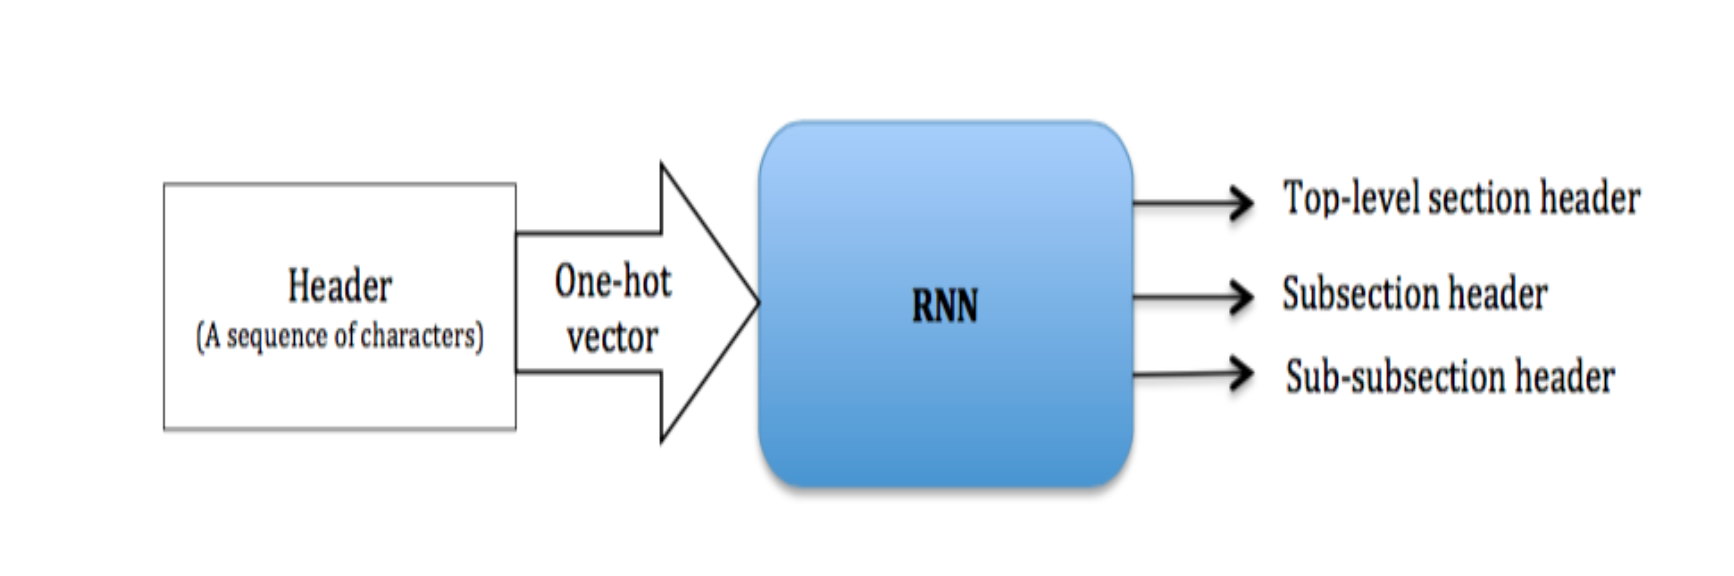
\includegraphics[width=0.7\textwidth]{pics/classifier.png}}
    \captionisp{Вход и выход классификатора заголовков}{Input and output of the section classifier}
    \label{fig:classifier}
\end{figure}

Классификатор (рис. \ref{fig:classifier}), который был использован при решении задачи, состоит из нескольких частей. Сначала строки документа подаются на вход классификатору (классификатор строк), который определяет, является ли строка заголовоком, затем строки-заголовки классифицируются точнее другими классификаторами (классификаторы секций). В этом решении структура документа имела вложенность 3, то есть предполагалось выделение секций, подсекций, подподсекций.
Кроме того, в данной работе был размечен датасет, на котором происходило обучение модели. Метрика качества - F1-мера, при идентификации заголовков итоговый score -- 0,96; при классификации секций средний F1-score -- 0,81.

Данный подход ограничивает число уровней вложенности извлекаемой структуры и так же не позволяет извлекать элементы списков. Разработанный нами метод позволяет извлекать структуру без ограничения уровней вложенности.

\section{Набор данных и манифест}
\subsection{Описание данных}

Датасет представляет собой набор документов в виде изображений в формате JPEG, скачанный с сайта zakupki.gov.ru \cite{zakupki}. Набор данных доступен для изучения \cite{data}. 

Анализируемые документы являются сканированными копиями страниц текстов государственных закупок. Каждое изображение будем считать отдельным документом. Из рассмотрения удалены документы, содержащие изображения и таблицы.

Данный корпус имеет ряд специфических особенностей. Текст расположен в одной колонке, не выделен цветом, шрифт не меняется (меняется только его начертание или размер). Большая часть всех текстов написана на русском языке, редко встречаются латинские буквы. Так как содержимое документов представляет собой в основном договоры предприятий, в текстах встречается большое количество элементов списков (нумерованных и маркированных), зачастую списки имеют очень глубокий уровень вложенности (четвертый, пятый). Заголовков относительно немного, они могут быть пронумерованы и также иметь глубокий уровень вложенности, поэтому их можно спутать с элементами списков.

Поскольку сканированная копия может быть сделана с любой страницы документа, а не только первой, на некоторых страницах (которые мы считаем отдельным документом) могут отсутствовать заголовки или элементы списков.

Первоначально набор данных состоял из 5000 изображений, однако на большей части этих изображений присутствовали таблицы, рисунки, рамки и прочие нетекстовые элементы, которые не рассматриваются в данной работе. Поэтому в итоговый набор вошли только 600 изображений, удовлетворяющие необходимым требованиям.



\subsection{Разметка данных}
Для создания обучающего набора данных часто используют ручную разметку -- предлагают выполнить задачу классификации человеку-аннотатору. 

В книге \cite{pustejovsky2012natural} предлагается выполнять разметку обучающего корпуса в следующем порядке:


\begin{enumerate}
    \item Спецификация задания -- формальное определение задания и формата данных, используемое ПО и так далее. 
    \item \label{labelingPipeline2} Составление Манифеста -- инструкции для аннотаторов. 
    \item Разметка данных. Непосредственно разметка данных с учётом Манифеста
    \item Измерение согласованности аннотаторов. На этом шаге проверяется то, что размечающие понимают задание одинаково. Если это не так, то производится возврат к шагу \ref{labelingPipeline2}
    \item Вынесение решения по аннотациям -- если каждый пример размечался более чем 1 анотатором, возникает необходимость объединить их результаты. Мы пропустили этот шаг, так как каждый документ размечался одним аннотатором. 
\end{enumerate}
    Опишем эти шаги подробнее применительно к нашей задаче. 
    
    \subsubsection{Спецификация задания}
        Мы поставили нашу задачу как многоклассовую классификацию строк. Аннотаторам последовательно показывались изображения сканированного документа, одна из строк которого обведена в красную рамку. Аннотатору было необходимо отнести текст в рамке к одному из наперёд заданных классов. В нашей задаче выполнялась классификация на следующие классы: 
        \begin{itemize}
            \item Заголовок;
            \item Элемент списка;
            \item Простой текст;
            \item Другое (не текст). 
        \end{itemize}
        Таким образом, аннотатору ставилась задача классификации изображения. Для выполнения этого задания использовалась система собственной разработки \cite{labeler}. После разметки данные сохранялись в формате JSON, формат описан в Приложении.
        %TODO вставить пример
        
    \subsubsection{Манифест}
        В предыдущей секции мы определили задание для разметки как классификацию изображения на один из 
        нескольких классов. Теперь необходимо определить, чем должны руководствоваться аннотаторы, относя 
        изображение к тому или иному классу, в этом им помогает \textit{манифест} или инструкция для разметки.
        
        Как правило, невозможно полностью формально описать правила классификации (в противном случае нам нет необходимости использовать машинное обучение). 
        Поэтому в манифесте допустимо использование нестрого определённых понятий  и правил (например: \textit{жирный текст, выравнивание по центру, изображение синей печати}). При этом важно, чтобы все аннотаторы понимали задание одинаково. Для того, чтобы убедиться в этом, вычисляется согласованность. 
        
    \subsubsection{Согласованность}
        Для проверки одинакового и правильного понимания задания аннотаторами необходимо измерить их согласованность:
        \begin{enumerate}
            \item Предложить нескольким аннотаторам независимо выполнить разметку одного и того же множества заданий. 
            \item Вычислить специальную статистику, показывающую насколько согласована разметка. 
            \item В случае низкой согласованности рекомендуется разобрать спорные ситуации и обновить манифест,
            лучше прописав правила для спорных ситуаций и добавив примеров. 
        \end{enumerate}
        Хороший обзор о методах вычисления согласованности можно найти в статьях
        \cite{artstein2008inter} и \cite{bayerl2011determines}.
        Для проверки правильности разметки была посчитана специальная статистика Cohen's kappa, принимающая значения $\leq 1$. Чем ближе $\kappa$ к 1, тем выше согласованность. После разметки десяти документов (407 строк) двумя аннотаторами значение статистики $\kappa$ оказалось равным 0.975, что считается высоким уровнем согласованности. 
        
        После чего было решено размечать остальной корпус документов. В результате было размечено 600 документов (21350 строк) и отдельные JSON файлы были объединены в один (рис. \ref{fig:label}).
        
        Стоит отметить, что высокая согласованность ещё не означает, что задание выполнено "правильно".
        Так, если все аннотаторы будут всегда относить каждое изображение к классу \textit{"Простой текст"}, не обращая внимания на признаки и манифест, то 
        $\kappa$ будет равна 1, но вряд ли это можно назвать правильной разметкой. Такая проблема актуальна при
        использовании краудсорсинга. Обзор методов краудсорсинга можно найти в статье \cite{gilyzevTurdakov2018}. 


\section{Описание решения}

\subsection{Описание реализованного метода}

Первым шагом в решении задачи является выделение текста и рамок для строк документа с помощью методов OCR. Вторым шагом является составление вектора признаков для каждой строки документа. С помощью выделенной текстовой информации извлекаются различные текстовые признаки, описанные в главе 4.2. Для визуальных признаков используется информация из координат рамок (для отступов и высоты). В определении жирности шрифта используется само изображение документа и координаты рамок строк внутри изображения.

Таким образом, каждый документ представлен набором векторов признаков для строк, а тренировочные данные являются объединением данных для документов.
Следующим шагом в решении задачи является применение алгоритма машинного обучения, который на основе выделенных признаков распределит строки по классам. Схема пайплайна показана на рис. \ref{fig:pipeline}

\begin{figure}[ht]
    \center{
\includegraphics[width=0.9\textwidth]{pics/pipeline.png}}
    \captionisp{Пайплайн обработки документов}{Pipeline for documents processing}
    \label{fig:pipeline}
\end{figure}

\subsection{Выделение признаков}

Среди признаков, характеризующих строки документа, можно выделить следующие группы:

\begin{itemize}

  \item Признаки, основанные на регулярных выражениях.

  Данная группа признаков основывается на анализе начала и конца каждой строки. Такие признаки очень важны для выявления элементов списков различных типов, а также могут сигнализировать о конце заголовка или начале списка.

  Регулярные выражения позволяют выделить следующие признаки:
  \begin{itemize}

    \item[--] начинается ли строка с цифры или буквы со скобкой или точкой (также анализируются иерархические выражения вида 1.1.1);
    \item[--] начинается ли строка с тире (и других символов, характерных для маркированного списка);
    \item[--] состоит ли строка целиком из заглавных букв (характерно для некоторых заголовков);
    \item[--] начинается ли строка с заглавной (строчной) буквы;
    \item[--] начинается ли строка с конкретных слов типа «Раздел», «Секция», «Глава» и т. д.;
    \item[--] оканчивается ли строка символами вида «. , ; :»;
    \item[--] оканчивается ли строка строчной буквой.

  \end{itemize}

  \item Текстовые признаки.

  Данная группа признаков связана с подсчетом некоторых строковых характеристик, а именно:

  \begin{itemize}

    \item[--] количество букв в первом и втором словах строки;
    \item[--] количество слов в строке (строка разбивается на слова по пробелам);
    \item[--] количество символов в строке (длина строки).

  \end{itemize}

  \item Визуальные признаки.
  
  Данная группа признаков связана с графическим представлением текста в документе. То есть при анализе строки рассматривается не ее текст, а следующие признаки (первые три признака измеряются в пикселях):

  \begin{itemize}

    \item[--] отступ от левого края страницы;
    \item[--] высота текста строки (точнее высота ограничивающей ее рамки);
    \item[--] отступ от верхнего края страницы;
    \item[--] жирность шрифта различных уровней (подробнее см. в главе 4.2.1).
    
     \end{itemize}

\end{itemize}

Важно рассматривать не одну строку, а ее окрестность, для увеличения точности классификатора строк. Поэтому к признакам каждой строки добавляются признаки четырех предыдущих и последующих строк.

Для строк, которые начинаются с нумерации, определяется, есть ли в документе строка, предшествующая данной с нумерацией, меньшей данной на единицу.

И, наконец, для каждого документа вычисляется средний отступ от левого края страницы, средняя высота шрифта, средняя длина строки, среднее число слов в строках, среднее значение для жирности шрифта (ядро свертки 5), среднее число букв в первом слове каждой строки. Данные значения добавляются к признакам каждой строки документа.

\subsubsection{Определение жирности шрифта}
Рассмотрим более подробно способ определения жирности шрифта. Для этого использовались морфологические операции Dilation и Erosion \cite{operations} из библиотеки OpenCV \cite{opencv}. Данные операции с помощью комбинаций увеличения и сужения границ на изображении позволяют детектировать жирность текста.

При работе с текстом в качестве исходного изображения используется bounding box конкретной строки, полученный с помощью tesseract \cite{tesseract}. В данной работе функции erode и dilate запускались с параметром kernel, равным от 2 до 7 включительно (6 раз).

\section{Экспериментальная проверка метода}

\subsection{Подбор классификатора}

При решении задачи было опробовано множество методов машинного обучения, для лучших из них проведен анализ результатов. В анализе участвовало 4 классификатора:

\begin{itemize}

  \item алгоритм k ближайших соседей (\href{https://scikit-learn.org/stable/modules/generated/sklearn.neighbors.KNeighborsClassifier.html}{KNeighborsClassifier});
  \item логистическая регрессия (\href{https://scikit-learn.org/stable/modules/generated/sklearn.linear_model.LogisticRegression.html}{LogisticRegression});
  \item градиентный бустинг (\href{https://scikit-learn.org/stable/modules/generated/sklearn.ensemble.GradientBoostingClassifier.html}{GradientBoostingClassifier});
  \item экстра-градиентный бустинг (\href{https://xgboost.readthedocs.io/en/latest/}{XGBClassifier}).

\end{itemize}

Набор размеченных документов тремя способами был разбит на тренировочное и тестовое множества. Разбиение производилось по документам, то есть группа строк, относящихся к одному документу попадала целиком либо в тренировочное, либо в тестовое множество. На каждом разбиении было проведено обучение классификаторов и вычисление F1-score. Усредненные значения F1-score для каждого классификатора указаны в табл. \ref{tab:classifier_comparison}.
\begin{table}[ht]
\captionisp{Сравнение классификаторов}{Classifier comparison}
\begin{tabular}{cc}
 \toprule
    \textbf{Классификатор} & \textbf{F1-score} \\
    \midrule
        Nearest Neighbors & 0.89 \\
        Logistic Regression & 0.9 \\
        Gradient Boosting & 0.92 \\
        \bf XGBoost & \bf 0.95 \\
    \bottomrule
    \end{tabular}
    \label{tab:classifier_comparison}
\end{table}

В целом, все рассмотренные классификаторы показали хороший результат (табл. \ref{tab:classifier_comparison}), наилучший результат показал XGBClassifier, поэтому было решено выбрать его.

\subsection{Анализ значимости признаков}

Анализ значимости признаков был проведен с помощью библиотеки xgbfir \cite{xgbfir} . В табл. \ref{tab:features_importances} представлены первые 10 признаков с наивысшей значимостью (information gain). Это признаки, которые имеют наибольший вес при вычислении предсказания классификатора.

\begin{table}[ht]
    \captionisp{Значимость признаков}{Features importances}
    \begin{tabular}{p{0.8\textwidth}p{0.1\textwidth}}
    \toprule
    \textbf{Признак} & \textbf{Information gain} \\
    \midrule
        Число символов первого слова в строке & 22089 \\
        Индикатор, является ли строка продолжением списка & 2400 \\
        Жирность шрифта & 2368 \\
        Число слов в строке & 2263 \\
        Отступ от левого края страницы & 1157 \\
        Признак начала строки с выражения вида 1.1.1 (произвольный уровень вложенности, вместо цифр могут быть буквы) & 1519 \\
        Жирность шрифта (менее жирный шрифт) & 811 \\
        Индикатор, заканчивается ли предыдущая строка буквой & 611 \\
        Число букв в начале строки & 361 \\
        Тире в начале строки & 359 \\
    \bottomrule
    \end{tabular}
    \label{tab:features_importances}
\end{table}

С использованием данных о важности признаков, в признаковое пространство были добавлены новые признаки. Например, вместо одного признака, отвечающего за жирность шрифта, была добавлена целая группа признаков, отвечающая за различные уровни жирности шрифта. Для самых важных признаков к вектору признаков каждой строки документа были добавлены усреднённые значения данных признаков по документу. В табл. \ref{tab:features_importances} представлен итоговый список признаков и значения их важности.

\subsection{Результаты}

После настройки параметров XGBClassifier \cite{tuning} ($learning\_rate=0.1$, $n\_estimators=1000$, $max\_depth=7$, $min\_child\_weight=2$,
$gamma=0$, $subsample=1$, $colsample\_bytree=1$, $alpha=0.01$) итоговый F1-score, полученный в результате кросс-валидации (разбиение данных на 3 части) оказался равным 0.98995. 

\subsection{Анализ ошибок}

На рис. \ref{fig:confusion_matrix} показана \href{https://en.wikipedia.org/wiki/Confusion_matrix}{матрица ошибок} для полученного классификатора. Матрица получена на валидационном датасете. По вертикальной оси расположены правильные классы, по горизонтальной - классы, которые предсказал классификатор. В клетках на пересечении расположены значения количества строк, у которых совпали данные классы.

\begin{figure}[ht]
  \center{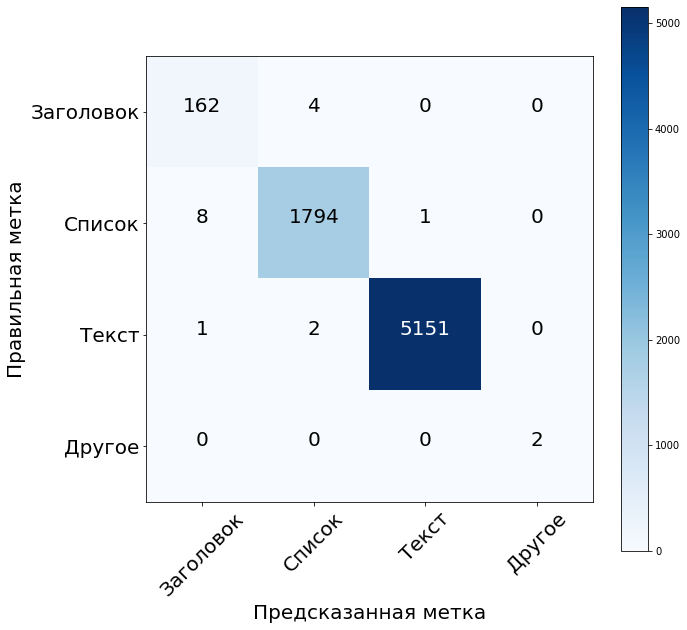
\includegraphics[width=0.6\textwidth]{pics/conf_matrix_rus.png}}
  \captionisp{Матрица ошибок без нормализации}{Confusion matrix without normalization}
    \label{fig:confusion_matrix}
\end{figure}

На рисунке видно, что 8 строк, относящихся к типу «Список», были проклассифицированы как «Заголовок», 4 строки, напротив, вместо метки «Заголовок» получили метку «Список». Аналогичную статистику можно посмотреть и для других пар классов.

Таким образом, больше всего классификатор путает классы «Заголовок» и «Список». Это можно объяснить тем, что некоторые признаки данных классов очень похожи, например, многие заголовки начинаются с нумерации, а элементы списков имеют большой отступ от левого края страницы.

\section{Заключение}
% был разработан метод, реализация - это кодирование
% нужно про пайплайн упомянуть и про разметку в нем
В данной статье разработан метод выделения логической структуры документа, основанный на классификации строк документа, определяющий в документах заголовки и списки разных уровней вложенности.
Реализован пайплайн, состоящий из обработки документов с помощью программы Tesseract \cite{tesseract} и применения к ним ручной разметки, выделения векторов признаков и обучения классификатора. Размеченный датасет доступен для изучения \cite{data}. Для эффективной классификации списков и заголовков помогает извлечение признаков, указанных в табл. \ref{tab:features_importances} и использование XGBClassifier \cite{xgb}. Итоговый F1-score на данных кросс-валидации, полученный при настройке параметров классификатора, равен 0.98995. Однако, в силу особенностей датасета классификатор может путать заголовки и элементы списков.

Дальнейшие исследования могут быть направлены на выделение более подробной структуры. Помимо классификации каждой строки можно определять её уровень вложенности по отношению к документу.

% \begin{otherlanguage}{english}
\printbibliography
% \end{otherlanguage}

{\vskip 12pt\normalfont\sffamily\bfseries\large Приложение / Appendix}
\setlength{\parskip}{6pt}

\begin{figure}[ht]
    \centering
    \begin{lstlisting}[language=Python,frame=none,basicstyle=\ttfamily]
    [
        {
        "name": name of the first document,
        "width": image width (pixels),
        "height": image height,
        "entities": [
            {
                "label": first line label,
                # bounding box for the first line
                "x": first line left indent,
                "y": first line top indent,
                "width": first line width,
                "height": first line height,
                "text": first line text
            }, ...
        }, ...
    ]
    \end{lstlisting}
    \captionisp{Результат разметки}{Labeling result}
    \label{fig:label}
\end{figure}

Выделяются следующие типы строк: заголовок, элемент списка, текст.

\begin{enumerate}
	\item Заголовок -- это название главы, секции, подглавы, параграфа. Строка помечается заголовком, если:
	\begin{itemize}
		\item текст визуально (полностью) выделяется жирностью (рис. \ref{fig:1});
		
		\begin{figure}[ht]
		    \frame{
\includegraphics[width=1.0\textwidth]{manifest/1.png}}
		    \captionisp{Пример заголовка №1}{Header example №1}
		    \label{fig:1}
		\end{figure}
		
		\item текст полностью выделяется шрифтом (курсив, подчеркнутый, другой шрифт, другой размер шрифта) (рис. \ref{fig:2});
		
		\begin{figure}[ht]
		    \frame{
\includegraphics[width=1.0\textwidth]{manifest/2.png}}
		    \captionisp{Пример заголовка №2}{Header example №2}
		    \label{fig:2}
		\end{figure}
		
		при этом если текст строки выделен шрифтом частично, то заголовком это не считается;
		
		\item текст выделяется отступом (расположен по центру) (рис. \ref{fig:3});
		
		\begin{figure}[ht]
		    \frame{
\includegraphics[width=1.0\textwidth]{manifest/3.png}}
		    \captionisp{Пример заголовка №3}{Header example №3}
		    \label{fig:3}
		\end{figure}
		
		\item если заголовок занимает несколько строк, остальные строки тоже относятся к типу «заголовок».
	\end{itemize}
	
	\item Элемент списка - это начало нумерованного или маркированного списка. Строка помечается как элемент списка, если:
	\begin{itemize}
		\item строка наряду с несколькими другими строками пронумерована («1. 1) а) 1.1» и т. д. в начале строки) или выделена некоторым маркером (точка, тире и т. д.);
		
		\item если элемент списка визуально занимает несколько строк, все строки кроме первой помечаются как текст. Также к списку не относятся строки, помеченные как заголовок (выделенные шрифтом, жирностью и т. д.).
		
		На рис. \ref{fig:4} как элемент списка будут помечены только две строки, остальные помечаются как текст.
		
		\begin{figure}[ht]
		    \frame{
\includegraphics[width=1.0\textwidth]{manifest/4.png}}
		    \captionisp{Пример элементов списка}{List example}
		    \label{fig:4}
		\end{figure}
		
	\end{itemize}
	
	\item Текстовые строки -- это все остальные строки, содержащие текст документа.
	\item Other -- при разметке могут попадаться выделенные области, не содержащие текста, такие области помечаются как «Other».
	
\end{enumerate}

\end{document}